\documentclass[14pt]{extarticle}
\usepackage[left = 3cm, right = 3cm, top = 3cm, bottom = 3cm]{geometry}
\usepackage{graphicx}
\usepackage{amsmath}

\usepackage{listings}
\lstset{ 
	language=Matlab,                		% choose the language of the code
	numbers=left,                  			% where to put the line-numbers
	numberstyle=\footnotesize,      		% the size of the fonts that are used for the line-numbers
	stepnumber=1,                   			% the step between two line-numbers. If it's 1 each line will be numbered
	numbersep=5pt,                  		% how far the line-numbers are from the code
%	backgroundcolor=\color{white},  	% choose the background color. You must add \usepackage{color}
	showspaces=false,               		% show spaces adding particular underscores
	showstringspaces=false,         		% underline spaces within strings
	showtabs=false,                 			% show tabs within strings adding particular underscores
%	frame=single,	                			% adds a frame around the code
%	tabsize=2,                				% sets default tabsize to 2 spaces
%	captionpos=b,                   			% sets the caption-position to bottom
	breaklines=true,                			% sets automatic line breaking
	breakatwhitespace=false,        		% sets if automatic breaks should only happen at whitespace
	escapeinside={\%*}{*)}          		% if you want to add a comment within your code
}

\begin{document}

\begin{flushleft}
\begin{LARGE}
\textbf{1.2}
\end{LARGE}
\end{flushleft}

\vfill
\begin{center}
\begin{Huge}Ordinary Differential Equations\end{Huge}
\end{center}
\vfill

\pagebreak

\begin{center}
\textbf{Question 1}
\end{center}

\begin{table}[h!]
\caption{Iterates with $h=0.4$}
\centering
\begin{tabular}{cccc}
\\
$x_n$ & $Y_n$ & $y(x_n)$ & $E_n$ \\ [0.5ex]
  0  &    0            &    0            &    0            \\ 
0.4  &    1.200000     &    4.684235e-01 &    7.315765e-01 \\ 
0.8  &   -2.231232     &    4.085668e-01 &   -2.639799e+00 \\ 
1.2  &    9.418332     &    2.929645e-01 &    9.125367e+00 \\ 
1.6  &   -3.164703e+01 &    2.002350e-01 &   -3.184726e+01 \\ 
  2  &    1.111734e+02 &    1.349998e-01 &    1.110384e+02 \\ 
2.4  &   -3.870770e+02 &    9.065022e-02 &   -3.871677e+02 \\ 
2.8  &    1.350038e+03 &    6.079639e-02 &    1.349977e+03 \\ 
3.2  &   -4.707051e+03 &    4.075944e-02 &   -4.707092e+03 \\ 
3.6  &    1.641270e+04 &    2.732317e-02 &    1.641267e+04 \\ 
  4  &   -5.722762e+04 &    1.831553e-02 &   -5.722764e+04 \\ 
4.4  &    1.995411e+05 &    1.227732e-02 &    1.995411e+05 \\ 
4.8  &   -6.957592e+05 &    8.229742e-03 &   -6.957592e+05 \\ 
5.2  &    2.425971e+06 &    5.516563e-03 &    2.425971e+06 \\ 
5.6  &   -8.458865e+06 &    3.697864e-03 &   -8.458865e+06 \\ 
  6  &    2.949434e+07 &    2.478752e-03 &    2.949434e+07 \\ 
6.4  &   -1.028408e+08 &    1.661557e-03 &   -1.028408e+08 \\ 
6.8  &    3.585847e+08 &    1.113775e-03 &    3.585847e+08 \\ 
7.2  &   -1.250312e+09 &    7.465858e-04 &   -1.250312e+09 \\ 
7.6  &    4.359583e+09 &    5.004514e-04 &    4.359583e+09 \\ 
  8  &   -1.520098e+10 &    3.354626e-04 &   -1.520098e+10 \\ 
8.4  &    5.300271e+10 &    2.248673e-04 &    5.300271e+10 \\ 
8.8  &   -1.848096e+11 &    1.507331e-04 &   -1.848096e+11 \\ 
9.2  &    6.443936e+11 &    1.010394e-04 &    6.443936e+11 \\ 
9.6  &   -2.246869e+12 &    6.772874e-05 &   -2.246869e+12 \\ 
 10  &    7.834375e+12 &    4.539993e-05 &    7.834375e+12 \\ 
\end{tabular}
\label{table:1}
\end{table}

\noindent \textbf{Growth rate}. To calculate the growth rate $\gamma$ we use $|E| = Ae^{{\gamma}x}$. Taking the natural log of both sides we have $log(|E|) = {\gamma}x + log(A)$. Plotting this graph and using the gradient function on Matlab we obtain that $\gamma$ is approximately $3.12$ to $3$ s.f. 

\pagebreak

\begin{table}[h!]
\caption{Iterates with $h=0.2$}
\centering
\begin{tabular}{cccc}
\\
\textbf{$x_n$} & \textbf{$Y_n$} & $y(x_n)$ & $E_n$ \\ [0.5ex]
0    &    0            &    0            &    0            \\ 
0.2  &    6.000000e-01 &    3.694018e-01 &    2.305982e-01 \\ 
0.4  &    2.247690e-02 &    4.684235e-01 &   -4.459466e-01 \\ 
0.6  &    1.368421e+00 &    4.580937e-01 &    9.103273e-01 \\ 
0.8  &   -1.508423e+00 &    4.085668e-01 &   -1.916990e+00 \\ 
$\vdots$ & $\vdots$ & $\vdots$ & $\vdots$ \\
9.2  &   -4.419109e+13 &    1.010394e-04 &   -4.419109e+13 \\ 
9.4  &    9.194507e+13 &    8.272407e-05 &    9.194507e+13 \\ 
9.6  &   -1.913032e+14 &    6.772874e-05 &   -1.913032e+14 \\ 
9.8  &    3.980302e+14 &    5.545160e-05 &    3.980302e+14 \\ 
 10  &   -8.281515e+14 &    4.539993e-05 &   -8.281515e+14 \\ 
\end{tabular}
\label{table:2}
\end{table}

\begin{table}[h!]
\caption{Iterates with $h=0.1$}
\centering
\begin{tabular}{cccc}
\\
\textbf{$x_n$} & \textbf{$Y_n$} & $y(x_n)$ & $E_n$ \\ [0.5ex]
0    &    0            &    0            &    0            \\ 
0.1  &    3.000000e-01 &    2.345174e-01 &    6.548263e-02 \\ 
0.2  &    3.029025e-01 &    3.694018e-01 &   -6.649934e-02 \\ 
0.3  &    5.489165e-01 &    4.396240e-01 &    1.092925e-01 \\ 
0.4  &    3.082602e-01 &    4.684235e-01 &   -1.601633e-01 \\ 
$\vdots$ & $\vdots$ & $\vdots$ & $\vdots$ \\
9.6  &   -6.108669e+14 &    6.772874e-05 &   -6.108669e+14 \\ 
9.7  &    9.022705e+14 &    6.128350e-05 &    9.022705e+14 \\ 
9.8  &   -1.332683e+15 &    5.545160e-05 &   -1.332683e+15 \\ 
9.9  &    1.968417e+15 &    5.017468e-05 &    1.968417e+15 \\ 
 10  &   -2.907417e+15 &    4.539993e-05 &   -2.907417e+15 \\ 
\end{tabular}
\label{table:3}
\end{table}

\pagebreak

\begin{table}[h!]
\caption{Iterates with $h=0.05$}
\centering
\begin{tabular}{cccc}
\\
\textbf{$x_n$} & \textbf{$Y_n$} & $y(x_n)$ & $E_n$ \\ [0.5ex]
0    &    0            &    0            &    0            \\ 
0.05 &    1.500000e-01 &    1.324987e-01 &    1.750133e-02 \\ 
0.1  &    2.253688e-01 &    2.345174e-01 &   -9.148545e-03 \\ 
0.15 &    3.313037e-01 &    3.118963e-01 &    1.940735e-02 \\ 
0.2  &    3.510597e-01 &    3.694018e-01 &   -1.834205e-02 \\ 
$\vdots$ & $\vdots$ & $\vdots$ & $\vdots$ \\
9.8   &   -7.443659e+14 &    5.545160e-05 &   -7.443659e+14 \\ 
9.85  &    9.079804e+14 &    5.274719e-05 &    9.079804e+14 \\ 
9.9   &   -1.107558e+15 &    5.017468e-05 &   -1.107558e+15 \\ 
9.95  &    1.351004e+15 &    4.772763e-05 &    1.351004e+15 \\ 
 10   &   -1.647960e+15 &    4.539993e-05 &   -1.647960e+15 \\ 
\end{tabular}
\label{table:4}
\end{table}
\noindent With $\gamma \approx 3.66,\;3.90,\;3.97\; $ for $h=0.2,\;0.1,\;0.05$ respectively.\\

\noindent \textbf{Instability}. As $h$ decreases from $0.4$ to $0.1$ the size of the instability increases. However, as $h$ decreases further to $0.05$ it decreases. As $h$ decreases the growth rate increases at a decreasing rate. Calculations with smaller values of $h$ (omitted) show that $\gamma$ tends to 4. 
\\
\begin{center}
\textbf{Question 2}
\end{center} 
\hfill

\noindent \textbf{i)} Rearranging the equation we have

\[Y_{n+1}+8hY_n-Y_{n-1} = 6he^{-hn}\]
We first look for complementary solutions satisfying 

\[Y_{n+1}+8hY_n-Y_{n-1} = 0\]
We try $Y_n = k^n$ to obtain

\begin{align*}
k^2 + 8hk - 1 &= 0\\
k &= -4h \pm \sqrt{16h^2+1}\\
\end{align*}
For the particular integral, we try $Y_n = Ae^{-nh}$

\begin{align*}
Y_{n+1}+8hY_n-Y_{n-1} &  = 6he^{-hn}\\
Ae^{-(n+1)h}+8Ahe^{-nh}-Ae^{-(n-1)h} &= 6he^{-hn}\\
A &= \frac{6h}{e^{-h}+8h-e^{h}}
\end{align*}
The full solution is

\[Y_n = C_1\left(-4h+\sqrt{16h^2+1}\right)^n+C_2\left(-4h-\sqrt{16h^2+1}\right)^n+\frac{6he^{-nh}}{e^{-h}+8h-e^{h}}\]
Applying the conditions $Y_0 = 0, Y_1 = 3h$ gives

\[C_1 = \frac{-3h}{e^{-h}+8h-e^{h}}\left[\frac{e^h+e^{-h}}{2\sqrt{16h^2+1}}+1\right], C_2 = \frac{-3h}{e^{-h}+8h-e^{h}}\left[-\frac{e^h+e^{-h}}{2\sqrt{16h^2+1}}+1\right]\]\\
\textbf{ii)} Using the binomial expansion for small $h$ gives

\[-4h+\sqrt{16h^2+1} = -4h + (1+ 8h^2 + O(h^4)) = e^{-4h}+O(h^3)\]
\[-4h-\sqrt{16h^2+1} = -4h - (1+ 8h^2 + O(h^4)) = -e^{4h}+O(h^3)\]
For large $n$ the second term (proportional to $e^{4nh}$) dominates the solution, causing the oscillatory motion and the instability.\\

\noindent \textbf{iii)} In the limit $h \rightarrow 0,\; n \rightarrow \infty$, keeping $nh \equiv x$ fixed

\[\lim_{h\to 0} \frac{6h}{e^{-h}+8h-e^h} = \lim_{h\to 0} \frac{6}{-e^{-h}+8-e^h} = 1\]\\
by L'Hopital's Rule. So $C_1 \rightarrow -1, C_2 \rightarrow 0$. From (ii) we have 

\[\left(-4h+\sqrt{16h^2+1}\right)^n \rightarrow e^{-4x}\]
Combining all of this together, we have

\[Y_n \rightarrow e^{-x}-e^{-4x}\] 
as required. The instability can be suppressed for a sufficiently small value of $h$ for a specific value of $x$. As $n$ gets larger (for bigger values of $x$) the solution will be unstable.

\begin{center}
\textbf{Question 3}
\end{center}
\vspace{-5mm}

\begin{table}[h!]
\caption{Numerical Solution with $h = 0.4$}
\centering
\begin{tabular}{ccc}
\\
\textbf{$x_n$} & \textbf{$Y_n\;(Euler)$} & $Y_n\;(RK4)$ \\ [0.5ex]
0   &   0        &          0 \\
0.4 &   1.200000 &   0.405856 \\
0.8 &   0.084384 &   0.381797 \\
1.2 &   0.488564 &   0.285601 \\
1.6 &   0.068294 &   0.199468 \\
  2 &   0.201299 &   0.135877 \\
2.4 &   0.041623 &  0.0916678 \\
2.8 &   0.083888 &  0.0616054 \\
3.2 &   0.022639 &  0.0413382 \\
3.6 &   0.035331 &  0.0277214 \\
  4 &   0.011590 &  0.0185854 \\
\end{tabular}
\label{table:5}
\end{table}

\begin{figure}[htp!]
\centering
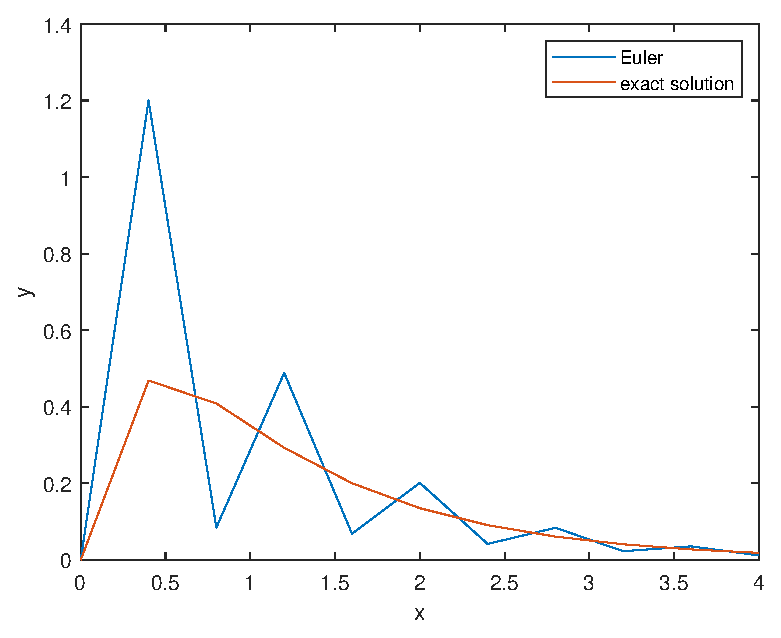
\includegraphics[scale=0.9]{Euler.eps}\\
\caption{The Euler Method with $h = 0.4$}
\label{figure:1}
\end{figure}

\begin{figure}[htp!]
\centering
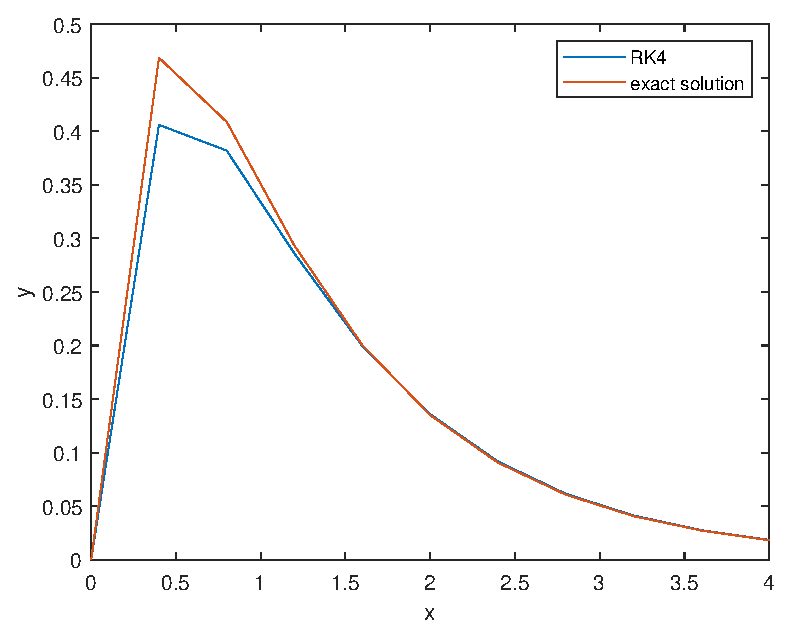
\includegraphics[scale=0.9]{RK4.eps}\\
\caption{The RK4 Method with $h = 0.4$}
\label{figure:2}
\end{figure}

\pagebreak
\begin{center}
\textbf{Question 4}
\end{center}

\begin{table}[h!]
\caption{Global error at $x_n=0.4$ for step length $h=0.4/2^k$}
\centering
\begin{tabular}{cccc}
\\
$k$ & $Euler$ & $LF$ & $RK4$ \\ [0.5ex]
0   &      0.731576 &        0.731576 &      -0.0625675 \\ 
  1 &      0.142815 &       -0.445947 &     -0.00192328 \\ 
  2 &     0.0637159 &       -0.160163 &    -8.42012e-05 \\ 
  3 &     0.0300389 &      -0.0447985 &    -4.41336e-06 \\ 
  4 &     0.0145986 &      -0.0115398 &    -2.52684e-07 \\ 
  5 &    0.00719827 &     -0.00290699 &    -1.51165e-08 \\ 
  6 &    0.00357439 &    -0.000728136 &    -9.24353e-10 \\ 
  7 &    0.00178107 &    -0.000182121 &    -5.71445e-11 \\ 
  8 &   0.000889015 &    -4.55357e-05 &    -3.55199e-12 \\ 
  9 &   0.000444128 &    -1.13843e-05 &    -2.21601e-13 \\ 
 10 &   0.000221969 &    -2.84609e-06 &    -1.39333e-14 \\ 
 11 &   0.000110961 &    -7.11523e-07 &    -1.05471e-15 \\ 
 12 &   5.54745e-05 &    -1.77881e-07 &    -5.55112e-17 \\ 
 13 &   2.77358e-05 &    -4.44702e-08 &      -4.996e-16 \\ 
 14 &   1.38675e-05 &    -1.11176e-08 &     1.16573e-15 \\ 
 15 &   6.93367e-06 &    -2.77939e-09 &    -5.55112e-16 \\ 
\end{tabular}
\label{table:6}
\end{table}

\noindent \textbf{Accuracy}. The global error of the Euler, Leapfrog and RK4 methods is $O(h),\; O(h^2),\; O(h^4)$ respectively$^1$. The graphs are straight lines, implying $|E_n| \propto h^k$, where $k$ is the gradient. Measuring the gradients of the straight sections of the graphs gives 1,2,4, as expected.

\begin{figure}[htp!]
\centering
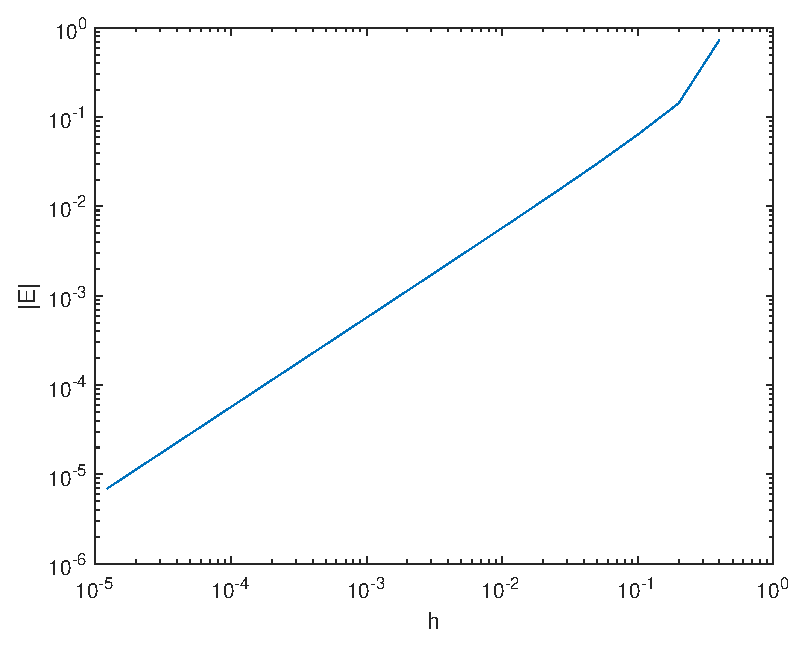
\includegraphics[scale=0.9]{ErrorEuler.eps}
\caption{log-log plot of $|E_n|$ against $h$ for the Euler method}
\label{figure:3}
\end{figure}

\begin{figure}[htp!]
\centering
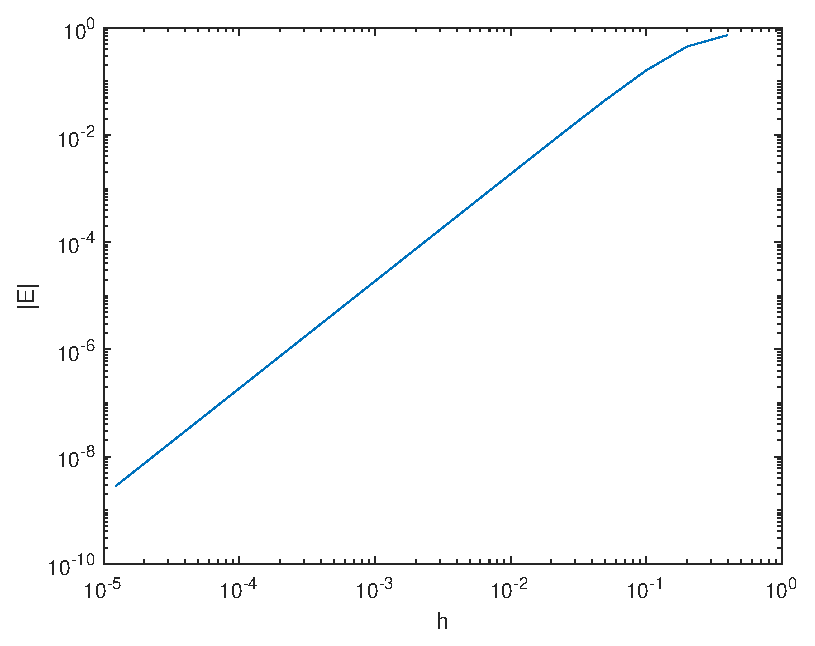
\includegraphics[scale=0.9]{ErrorLF.eps}
\caption{log-log plot of $|E_n|$ against $h$ for the LF method}
\label{figure:4}
\end{figure}

\begin{figure}[htp!]
\centering
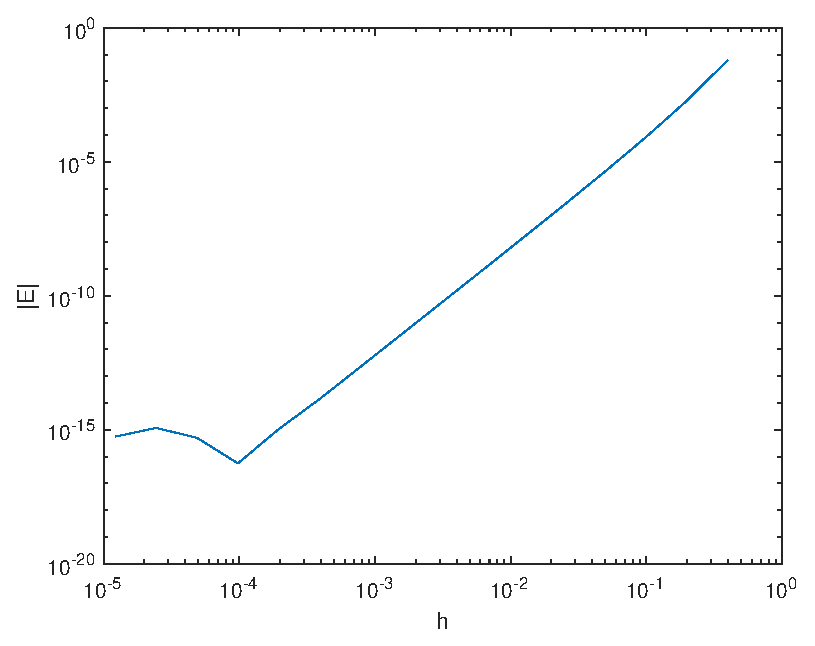
\includegraphics[scale=0.9]{ErrorRK4.eps}
\caption{log-log plot of $|E_n|$ against $h$ for the RK4 method}
\label{figure:5}
\end{figure}

\pagebreak
\begin{center}
\textbf{Question 5}
\end{center}
\vspace{-5mm}

\[\frac{d^2y}{dt^2} + \gamma\frac{dy}{dt} + \Omega^2y = a\sin(\omega t)\]
For the complementary function, we try $y_c = Ae^{mx}$:

\[m^2+\gamma m+\Omega^2 = 0\]
\[m_1 = \displaystyle{\frac{-\gamma + \sqrt{\gamma^2 -4\Omega^2}}{2}},\;\; m_2 = \displaystyle{\frac{-\gamma - \sqrt{\gamma^2 -4\Omega^2}}{2}}\]
For the particular integral, we try $y_p = C\sin(\omega t) +D\cos(\omega t)$ and find

\[C = \displaystyle{\frac{a(\Omega^2 - \omega^2)}{(\Omega^2 - \omega^2)^2 +\omega^2 \gamma^2}},\; D = \displaystyle{\frac{-a\omega \gamma}{(\Omega^2 - \omega^2)^2 +\omega^2 \gamma^2}}\]
So the full solution is 

\begin{equation} \label{eq:1}
y = \displaystyle{\alpha_1e^{m_1t}+\alpha_2e^{m_2t}+C\sin(\omega t)+D\cos(\omega t)}
\end{equation}
where $\alpha_1$ and $\alpha_2$ are constants.\\

\noindent Since $0<\gamma<2\Omega,\; \sqrt{\gamma^2 -4\Omega^2}$ is imaginary. Then also since $-\gamma<0$, $e^{m_1t},\; e^{m_2t} \rightarrow 0$  as $t \rightarrow \infty$. 

\[y \rightarrow C\sin(\omega t)+D\cos(\omega t) = A_s\sin(\omega t - \phi_s)\]
where

\[A_s = a\left((\Omega^2-\omega^2)^2+\omega^2\gamma^2\right)^{-\frac{1}{2}},\; \phi_s =\arctan\left(\frac{\omega\gamma}{\Omega^2-\omega^2}\right)\]

\begin{center}
\textbf{Question 6}
\end{center}
The analytical solution is given by equation (1) with 
\[m_1 = \frac{-\gamma + \sqrt{\gamma^2 -4}}{2},\; m_2 = \frac{-\gamma - \sqrt{\gamma^2 -4}}{2},\; C = \frac{1 - \omega^2}{(1 - \omega^2)^2 +\omega^2 \gamma^2}\]

\[D = \frac{-\omega \gamma}{(1 - \omega^2)^2 +\omega^2 \gamma^2},\; \alpha_1 = \frac{m_2D-\omega C}{\sqrt{\gamma^2-4}},\;\alpha_2 = \frac{\omega C-m_1D}{\sqrt{\gamma^2-4}}\]

\noindent \textbf{Error}. As $h$ decreases, the error of the numerical solution decreases. This is as expected since $E_n = O(h^4)$ for the RK4 method, so decreasing the step size decreases the error.


\begin{table}[htp!]
\caption{Iterates with $h=0.4$}
\centering
\begin{tabular}{cccc}
\\
$t_n$ & $Y_n$ & $y(t_n)$ & $E_n$ \\ [0.5ex]
   0 &          0 &          0 &    0            \\ 
 0.4 &  0.0162971 &  0.0162278 &    6.928741e-05 \\ 
 0.8 &   0.107096 &   0.107052 &    4.408538e-05 \\ 
 1.2 &   0.277351 &   0.277357 &   -6.186866e-06 \\ 
 1.6 &   0.463176 &   0.463193 &   -1.746659e-05 \\ 
   2 &   0.570018 &   0.569982 &    3.616040e-05 \\ 
 2.4 &   0.525149 &   0.525017 &    1.323705e-04 \\ 
 2.8 &   0.319065 &   0.318849 &    2.157463e-04 \\ 
 3.2 &  0.0160156 &  0.0157863 &    2.292653e-04 \\ 
 3.6 &  -0.271422 &  -0.271568 &    1.461683e-04 \\ 
   4 &  -0.431911 &  -0.431897 &   -1.338605e-05 \\ 
 4.4 &  -0.405897 &  -0.405708 &   -1.889432e-04 \\ 
 4.8 &  -0.213414 &  -0.213108 &   -3.065759e-04 \\ 
 5.2 &  0.0540853 &  0.0543986 &   -3.132468e-04 \\ 
 5.6 &   0.274493 &   0.274696 &   -2.024369e-04 \\ 
   6 &   0.349891 &    0.34991 &   -1.877553e-05 \\ 
 6.4 &     0.2504 &   0.250239 &    1.608557e-04 \\ 
 6.8 &  0.0269379 &  0.0266766 &    2.613142e-04 \\ 
 7.2 &  -0.212968 &  -0.213211 &    2.427793e-04 \\ 
 7.6 &  -0.355165 &  -0.355284 &    1.184965e-04 \\ 
   8 &  -0.331653 &  -0.331601 &   -5.152503e-05 \\ 
 8.4 &  -0.151895 &  -0.151707 &   -1.880424e-04 \\ 
 8.8 &   0.101712 &   0.101941 &   -2.287525e-04 \\ 
 9.2 &   0.312064 &    0.31222 &   -1.565432e-04 \\ 
 9.6 &    0.38158 &   0.381587 &   -6.894475e-06 \\ 
  10 &   0.277415 &   0.277266 &    1.489114e-04 \\ 
\end{tabular}
\label{table:6}
\end{table}

\begin{table}[htp!]
\caption{Iterates with $h=0.2$}
\centering
\begin{tabular}{cccc}
\\
$t_n$ & $Y_n$ & $y(t_n)$ & $E_n$ \\ [0.5ex]
 0 &          0   &          0 &    0            \\ 
 0.2 & 0.00218298 & 0.00218072 &    2.253537e-06 \\ 
 0.4 &  0.0162308 &  0.0162278 &    2.943649e-06 \\ 
 0.6 &  0.0501524 &  0.0501499 &    2.537562e-06 \\ 
 0.8 &   0.107054 &   0.107052 &    1.578828e-06 \\ 
$\vdots$     & $\vdots$   & $\vdots$ & $\vdots$  \\
 9.2 &   0.312215 &   0.31222  &   -5.602516e-06 \\
 9.4 &   0.368444 &   0.368445 &   -9.474735e-07 \\ 
 9.6 &   0.381591 &   0.381587 &    3.872336e-06 \\ 
 9.8 &   0.349987 &   0.349978 &    8.266914e-06 \\ 
  10 &   0.277278 &   0.277266 &    1.169810e-05 \\ 
\end{tabular}
\label{table:7}
\end{table}

\begin{table}[htp!]
\caption{Iterates with $h=0.1$}
\centering
\begin{tabular}{cccc}
\\
$t_n$ & $Y_n$ & $y(t_n)$ & $E_n$ \\[0.5ex]
 0   &            0 &            0 &    0            \\ 
 0.1 &  0.000281107 &  0.000281035 &    7.142962e-08 \\ 
 0.2 &   0.00218084 &   0.00218072 &    1.179555e-07 \\ 
 0.3 &   0.00711216 &   0.00711202 &    1.427963e-07 \\ 
 0.4 &     0.016228 &    0.0162278 &    1.496598e-07 \\ 
$\vdots$     & $\vdots$   & $\vdots$ & $\vdots$      \\ 
 9.6 &     0.381587 &      0.381587 &   3.607877e-07 \\
 9.7 &     0.371272 &      0.371271 &   4.905502e-07 \\ 
 9.8 &     0.349979 &      0.349978 &   6.059597e-07 \\ 
 9.9 &     0.318333 &      0.318332 &   7.034446e-07 \\ 
  10 &     0.277267 &      0.277266 &   7.799768e-07 \\ 
\end{tabular}
\label{table:8}
\end{table}

\pagebreak
\begin{center}
\textbf{Question 7}
\end{center}

\begin{figure}[htp!]
\centering
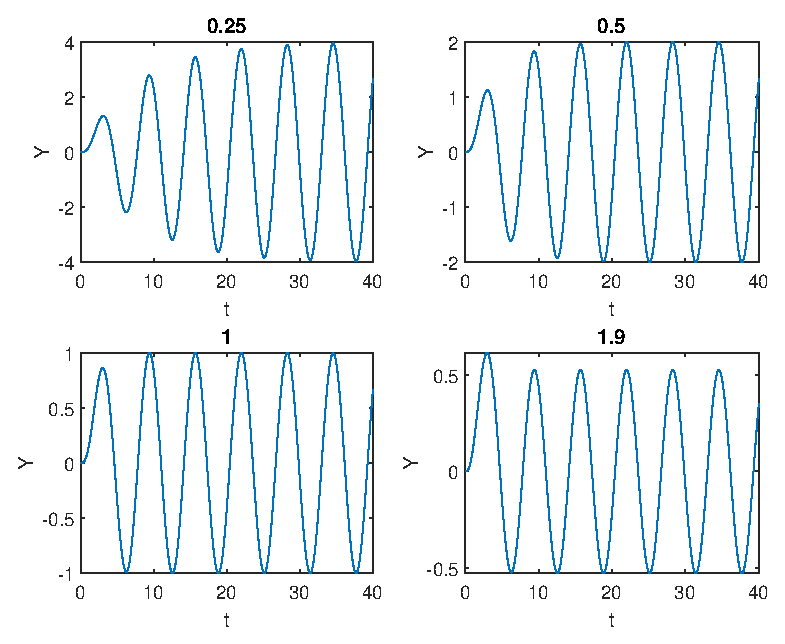
\includegraphics[scale=0.8]{Q7_w=1.eps}\\
\caption{Plots of the numerical solutions of $(20)-(21)$ with $\omega = 1$}
\label{figure:6}
\end{figure}


\begin{figure}[htp!]
\centering
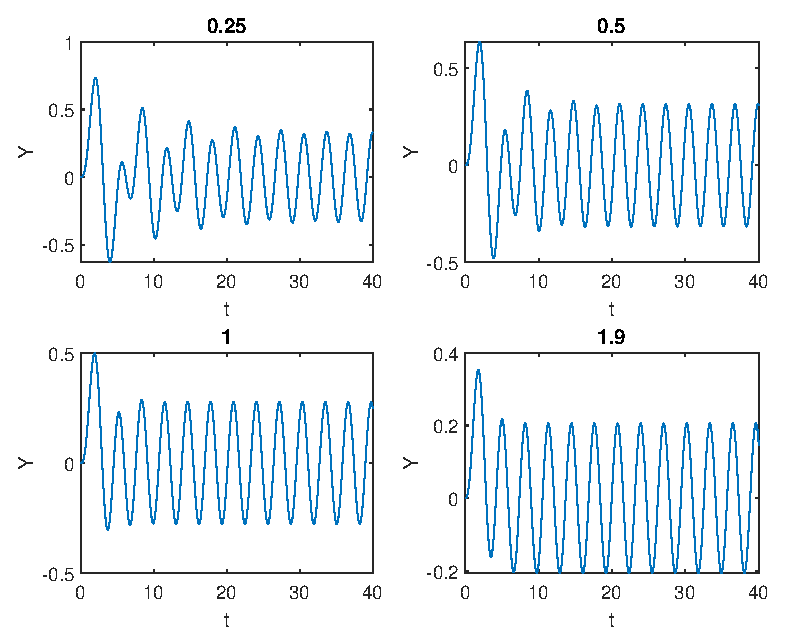
\includegraphics[scale=0.8]{Q7_w=2.eps}\\
\caption{Plots of the numerical solutions of $(20)-(21)$ with $\omega = 2$}
\label{figure:7}
\end{figure}

\noindent \textbf{Short-time response}. The system starts at rest, shown by the short horizontal line near $t=0$, in agreement with the initial conditions. In the complementary solution there is under-damping, caused by the $e^{-\gamma t/2}$ term. If there were no forcing the oscillations would gradually decrease in amplitude. The particular integral superposes onto this, creating the initial oscillations in the graphs, which are clearly distinct from those that occur later in time.\\

\noindent \textbf{Long-time response}. For large $t$ the complementary solution dies out and the behaviour is determined by the particular integral.
\[y \approx A_s\sin(\omega t - \phi_s),\; A_s = \left((1-\omega^2)^2+\omega^2\gamma^2\right)^{-\frac{1}{2}},\; \phi_s =\displaystyle{\arctan\left(\frac{\omega\gamma}{1-\omega^2}\right)} \]

\noindent Since $0<\gamma<2\Omega$. This is shown in the plots by the regular sinusoidal waves, demonstrating the system is oscillating in harmony with the driver. \\

\noindent \textbf{Damping}. Increasing $\gamma$ decreases the amplitude. Heavier damping takes away more energy from the system, causing it to oscillate with a smaller amplitude. We see that for large $t$ the amplitude is $O(1/\gamma)$.\\

\noindent \textbf{Frequency}. The frequency of the plots for $\omega = 2$ is twice that of the plots for $\omega = 1$. This is caused by the particular integral having the same frequency as that of the forcing. Having a driver that oscillates twice as quickly will cause the system to do so too.\\

\noindent \textbf{Resonance}. The amplitude is smaller for $\omega = 2$ than for $\omega = 1$ for any given amount of damping. The greatest amplitude is found by minimising
\[(1-\omega^2)^2+\omega^2\gamma^2 = \left(\omega^2 + \frac{\gamma^2 -2}{2}\right)^2+\gamma^2\left(1-\frac{\gamma^2}{4}\right)\]
which occurs at $\omega_r = \sqrt{1-\gamma^2/2}$, the resonant frequency. The amplitude diminishes as $\omega$ moves away from it. Since $\omega = 1$ is closer to $\omega_r$, it creates greater amplitudes than $\omega = 2$. Resonance occurs when the driving frequency is approximately equal to the natural frequency, $\sqrt{1-\gamma^2/4}$, causing the system to oscillate with a large amplitude.\\


\pagebreak
\begin{center}
\textbf{Question 8}
\end{center}
\noindent \textbf{Step size}. The value of $h$ used was 0.001. The same value was used in Q7 and provided sufficiently accurate results. 

\begin{figure}[htp!]
\centering
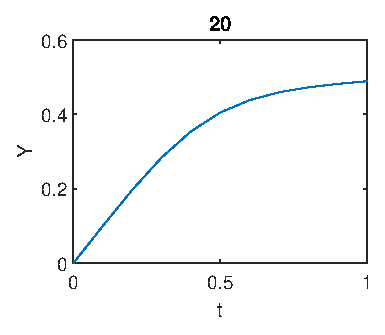
\includegraphics[scale=0.9]{Q8.eps}\\
\caption{Plots of the numerical solutions of $(22)-(23)$}
\label{figure:6}
\end{figure}

\noindent Using the hint and substituting (24) into (22) we have
\[\delta^{-1}(y_{-1}''+y_{-1})+(y_0''+y_0+y_{-1}^2y_{-1}'-\sin t)+\delta(y_1''+y_1+2y_{-1}y_{-1}'y_0+y_{-1}^2y_0')+\hdots = 0\]
Treating $\delta$ as a variable, all the coefficients must be 0. Using (25), $A = -\sqrt[3]{4},\, C = 1/8$ and $B$ is arbitrary.\\

\noindent In the plots for $\delta = 0.25,0.5,1.0$, the driver causes the system to begin oscillating with an increasing amplitude until it reaches the steady-state. $y_{-1}$ is the dominant term, from which we see the long-term amplitude is about $-\sqrt[3]{4}/\delta$, agreeing with the plots. These are similar to those for $\gamma = 0.25,0.5,1.0$ and $\omega = 1$. In both cases the damping is fairly light so the driver has the greatest effect on the system, leading to solutions that look the same.  \\

\noindent In the plot for $\delta = 20$ there are initially oval-shaped oscillations. This means the system has slow turns at the top and fast turns at the bottom. These become more sinusoidal later in time as the system moves more in harmony with the driver. The system is pulled 'down' gradually. The amplitude is also about $-\sqrt[3]{4}/\delta$.\\

\noindent For all plots we see that the frequency is the same as that of the driver. All systems eventually oscillate in harmony with the driver.\\
\\
\\
\\
\noindent \textbf{References}\\
$^1$ \textit{An Introduction
to Numerical Methods} by A.Kharab and R.B.Guenther - page 392


\pagebreak

\begin{center}
\textbf{Program} Euler.m \textbf{for Euler's method}
\end{center}
\lstinputlisting[language=Matlab]{Euler.m}

\begin{center}
\textbf{Program} Leapfrog.m \textbf{for LF method}
\end{center}
\lstinputlisting[language=Matlab]{Leapfrog.m}

\begin{center}
\textbf{Program} RK4.m \textbf{for RK4 method}
\end{center}
\lstinputlisting[language=Matlab]{RK4.m}

\begin{center}
\textbf{Program} RK4S2.m \textbf{for RK4 method for Q6,7,8}
\end{center}
\lstinputlisting[language=Matlab]{RK4S2.m}

\begin{center}
\textbf{Program} func.m \textbf{for section 1}
\end{center}
\lstinputlisting[language=Matlab]{func.m}

\begin{center}
\textbf{Program} func2.m \textbf{for Q6,7}
\end{center}
\lstinputlisting[language=Matlab]{func2.m}

\begin{center}
\textbf{Program} func3.m \textbf{for Q8}
\end{center}
\lstinputlisting[language=Matlab]{func3.m}


\end{document}

